\chapter{Introduction}
With the ever increasing need for storage and computational power,
governments, research institutes and industry are rushing to adopt
cloud computing, moving away from a model where computational projects
are executed on local computers.

The communities of researchers that need access to the computational
power required to carry out non-trivial simulations and analysis of
data are often distributed geographically, as are the computing
resources they rely on.

\highlight{something}


\section{Background}
To run computations effectively on modern supercomputers and computer
clusters the applications need strong scaling. When this is a
limitation for applications the available resources are not used to
reach highest possible performance.

%Copernicus paper

%Many interesting real-world applications (all that are not
%embarrassingly parallel) require some interprocess communication for
%scaling and are therefore limited both by the availability of this
%bandwith as well as the total amount of resources for high absolute
%performance.


Molecular dynamics simulations are computations which have limitations
as described, but there is a possibility due to the fact that many of
these computations are of statistical nature. Relying on sampling of
many individual simulations makes it possible to distribute the
workload on supercomputers and computer clusters. This is a
parallelization of such simulations which gives a great perfomance
boost when high numbers of cores are available.

The simple way of parallelizing can be generally described by a very
simple workflow. The workflow contains a simulation and an analysis
stage with a feedback. 

\begin{center}
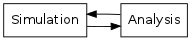
\includegraphics{Chapters/IntroductionIncludes/workflow.png}
\end{center}

The entire computation is initialized by generating a large number of
small simulations. Each simulation will send the result data to the
analysis stage. The analysis stage will analyze the data and create
some result of the computation so far. In this workflow the analysis
stage has a feedback to the simulation stage. This means the analysis
stage will generate new directed simulation depending on the current
result, i.e. what parts still needs more data. A computation like this
is highly parallel and modular which gives a possibility of using more
resources to spead up the entire computation.

An example of a described workflow would be a morkov stat
modeling. Where the different states are states in molecular
simulations. A large number of simulation states would start from
different states and would gather data for the analysis stage. The
result would be the different probabilities in the markov state
model. The feedback would be directed to the states that still need
more data.%(few simulations ended in that state)

\highlight{example figures ?}

%Molecular dynamics simulations pose significant computaional
%challanges. The systems are big enough to be parallelized, with
%100-500 particles assigned to each core in high-performance molecular
%dynamics (MD) packages such as Gromacs [10, 17] when run on a system
%with sufficiently low interconnect latency.

clouds are solutions to run computations on high-performing computer
systems. \citet{foster:2008} defines clouds as:

\begin{quote} \slshape
  A large-scale distributed computing paradigm that is driven by
  economies of scale, in which a pool of abstracted, virtualized,
  dynamically-scalable, managed computing power, storage, platforms,
  and services are deliviered on demand to externaal customers over
  the Internet.
\end{quote}

The resources are opaque to the user who use a pre-defined API to run
and use the system. This means the system can contain different kind
of computation power and the user is not affected. Running molecular
dynamics simulations on a cloud computing resource would need high
parallelization, such as described above, to achieve a perfomance
boost.

%cloud computing and Grid computing 360-Degree Compared:

%In a Cload, different levels of services can be offered to an end
%user, the user is only exposed to a pre-defined API, and the lower
%level resources are opaque to the user...

There are a few challenges when using clouds. Defining an API for
users to discover, request and use resources provided by the cloud can
be difficult. An API needs to have a good way of using the
computational power to execute the users projects. The users should
also be able to use all different features available in the cloud and
the API needs to be simple enough so that any user can understand it
without having knowledge of the cloud system behind the API.

The cloud needs to coordinate executions on the available resources
when the computations are often highly parallel. Executions may even
need to support different software and hardware.

%In this paper, we show that clouds and Grids share a lot commonality
%in their vision, architecture and technology, but they also differ in
%various aspects such as security, programming model, business model,
%compute model, data model, applications, and abstractions.

%Nevertheless,yes: the problems are mostly the same in clouds and
%Grids. There is a common need to be able to manage large facilities;
%to define methods by which consumers discover, request, and use
%resources provided by the central facilities; and to implement the
%often highly parallel computations that execute on those resources.

Monitoring progress and resources is a challenge since the users are
not in direct contact with the hardware which actually runs the
application. ``Essentially monitoring in clouds requires a fine
balance of business application monitoring, enterprise server
management, virtual machine monitoring, and hardware maintenance, and
will be a significant challenge for cloud computing as it sees wider
adoption and deployments.''\citep{foster:2008}

%Another challenge that virtualization brings to clouds is the
%potention difficulty in fine-control over the monitoring of
%resources.

%PROVENANCE

Provenance in this context is basically a trace of the computations
with all the necessary information (data sources, intermediate
states). This is very important for researchers, in order to track the
project and be able to recreate the results. Without this the an
experiment would not be as useful to the researchers as it could be,
for example to validate their findings. Users can save alot of
computation hours when having access to provenance information. In
some cases it is of great use to be able to change something and start
from an intermediate state of a computation instead of starting from
scratch. Provenance is a relatively unexplored area within cloud
computing and can be challanging to provide for general applications.

%``Provenance refers to the derivation history of a data product,
%including all the data sources, intermediate data products, and the
%procedures that were applied to produce the data product.''

%On the other hand, clouds are becoming the future playground for
%e-science research, and provenance management is extremely important
%in order to track the processes and support the reproducibility of
%scientific results.

%Provenance is still an unexplored area in cloud environments, in
%which we need to deal with even more challenging issues such as
%tracking data production across different service providers (with
%different platform visibility and access policies) and across
%different software and hardware abstraction layers within one
%provider.

One way of programming/using a cloud can be to use workflow
systems. The workflow can be represented as a graph of individual
executions of applications where the edges are dependencies and how
data are passed between the applications. Users can submit these
workflow schemes to the cloud using the API interface.

%PROGRAMMING MODEL

%More specifically, a workflow system allows the composition of
%individual (single step) components into a complex dependency graph,
%and it governs the flow of a data and/or control through these
%components.


%The data Grid...

%In an increasing number of scientific disciplines, large data
%collections are emergin as important community resources.


There is a cloud solution for running parallelized molecular
simulations and it is called Copernicus.


\subsection{Copernicus}
Copernicus is a software system that is made to distribute and
parallelize large molecular dynamics simulations. The system
integrates elements from distributed computing, and applies them to
more traditional high-performance compute clusters. By taking
advantage of the fast interconnects that may be available on these
compute environments, individual simulations are parallelized as far
as possible. This approach enables Copernicus to use
orders-of-magnitude more cores than a traditional simulation run on a
sumpercomputer, and it allows for larger-scale simulations than would
be possible with purely distributed systems, while it reduces
time-to-solution significantly.

The idea behind Copernicus is to exploit the inherent parallelism of
ensemble simulation and to make use of advanced sampling algorithms,
while keeping the performance advantages of massively parallel
simulations. Such computations are called projects in the system.

\begin{quote} \slshape
  A project is executed as a single job, but breaks it up into coupled
  individual parallel simulations over all available computational
  resoureces, with the single simulation as the individual work
  unit. While the software has been optimized for using multiple
  high-performance compute clusters, it works equally well with cloud
  computing instances or even individual
  workstations.\citep{pronk:2011}
\end{quote}

To handle projects with many simulations as a single entity Copernicus
needs to able to
\renewcommand{\labelitemi}{-}
\begin{itemize} \slshape
\item match and distribute the individual simulations to the available
  computational resources,
\item run simulations on a variety of remote platforms simultaneously:
  HPC clusters, workstations, cload copmuting instances, et cetera,
\item parallelize tasks to the maximum extent possible on each
  resource, and use adaptive coupling beyond this,
\item allow flexibility in the types of projects tat can be run,
\item perform real-time analysis of the running project.
\item enable monitoring of running projects.\citep{pronk:2011}
\end{itemize}

Copernicus network structure contains three components: clients,
servers and wrokers. The clients are user interfaces to interact with
the system. Users will send and start their computational project to a
server using the client. The server handels projects and controls the
work distribution. Jobs will be sent to available workers, depending
on which worker is best suited for the job. A worker will calculate
the jobs assigned to it and send the result back to the server. It
will also announce to servers when it is available. Multiple worker
processes can be run on the same system, e.g. supercomputers would run
a great number of wokers to use all the available cores.

Copernicus projects are described by building computational
\emph{data-flow networks}. Data-flow networks are networks which
describe how streams of data is sent between different executions.  A
network is a set of connections between black boxes, where a black box
can either be a function or another network. Both functions and
networks have external inputs and outputs which are used to connect
the networks between scopes. A function has a subnetwork and a
controller which both can't be accessed outside the function. The
subnetwork is a normal network where the controller can add
connections and black boxes. A controller is in itself a black box in
Copernicus. It has access to the networks defenition and has
permission to add new black boxes and connections.

%old defenition of controllers
%
%Controllers are basically event handlers that trigger in certain
%situations, e.q. they are called when a project starts, a subproject
%finishes, a command finishes, etc\citep{pronk:2011}.

A real life example project could be the following:

\begin{center}
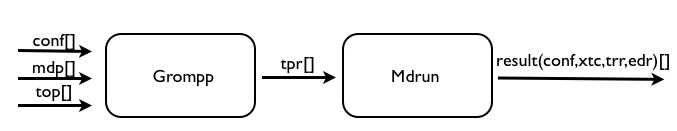
\includegraphics[scale=0.4]{Chapters/IntroductionIncludes/example.png}
\end{center}

In this project Grompp takes inputs and generates topology files. The
list \emph{conf[]} is the configurations for each simulation. Mdrun
then takes the topology files as inputs and runs the simulations. Even
though this example does not have a feedback to generate more
simulations, the Copernicus system is still very useful. When having
access to limit computation hours on different systems, users could
just split the list \emph{conf[]} and split up the jobs, while just
repeating the same workflow with different inputs, and still get the
same data. If this was not possible the user would need save the state
of the computation and send potentially very large amount of data
between the systems.

%There are primitive types like files, strings, ints, etc. There are
%also compound types lists, dictionaries and function types
\highlight{types, monitoring, provenance?}

The problem with Copernicus was the lack of a good way to describe
projects. There were no intuitive way of giving input to the system,
and that is why this project was formed.


\section{Problem statement}
The objective is to find and implement a solution for the need of a
new way of giving Copernicus information of the users projects. The
developers specifically stated that the wanted a domain-specific
language(DSL) for this solution, and that they later on want to add a
graphical solution using this DSL.

The DSL should allow users of Copernicus to define their computational
projects. The projects should be able to be defined as piping
computations in a data-flow network, which means that the DSL needs to
be able to describe data-flow networks in plain text.

The intended users are assumed to possess some knowledge of
programming, but are not necessarily adept programmers. The design of
the DSL should therefore be simple and intuitive. The DSL needs to be
easy to understand so it becomes an asset instead of an hindrance.

The DSL should be fully functional in Copernicus. The users needs to
be able to use all the features and properties available in
Copernicus.

Copernicus has function libraries which needs to be usable in the
language. This implies a certain amount of flexibility since there are
not a static amount of libraries, as new ones can be added. The DSL
should be able to cope with any new plug-ins.

The implementation should have an output of a form so that it can
easilly be integrated in the Copernicus system. The implementation
also needs to be easy to install on any system, supercomputer or
other.

\subsection{Delimitations}
The most important part of the project is to have a working
implementation. There are features which can be added to the DSL for
describing even more advanced projects with better syntax, e.g. simple
arithmetics.

The implementation generates XML code since Copernicus already has
support for reading XML files describing computational projects. This
will most likely be replaced by building the projects directly from
the abstract syntax trees, rendering the XML generation
redundant. This step would require much more understanding of how
Copernicus work, which is not within the time limit of this project.

This project has not considered a graphical solution at all. Graphical
implementations of related work has only been used get inspiration for
the DSL. A graphical interface would be good addition, but it is
another project. Such a solution can use many parts of the developed
DSL implementation.

The language we chose to write the implementation in is Python. This
choice was based on formost an easy implementation and maintenance,
since Copernicus is written in Python. It would have been possible to
use effective tools and another language, but instead tools
specifically for python were used.


\section{Related work}

\highlight{hadoop -> map reduce}


\section{Remaining chapters}
The chapters in the next part will cover the different parts of the
project in a fashion fairly close to the different stages the project
went through.

The research conducted to gather domain knowledge is presented in
\autoref{chap:research}. In \autoref{chap:language}, the language, its
features and various design choices will be covered. The actual
implementation details are described in \autoref{chap:implementation}.
